% \documentclass[dvips,ruledheader,a4]{abnt}
\documentclass{abnt}
\usepackage[brazil]{babel}
\usepackage[latin1]{inputenc}
\usepackage[pdftex]{graphicx}
\usepackage{abnt-alf}
\usepackage{latexsym}
\usepackage{psfrag}
\usepackage[center]{caption2}

% \newcommand{\lombadassss}{\vec{\mathbf{p}}}

\newcommand{\epigrafe}[1]{
\vspace{1cm}{\raggedright\par\sffamily\slshape #1\par}
}



\newcommand{\lombada}{
\begin{titlepage}
\espaco{1.1}

\begin{center}
	\large\ABNTchapterfont\ABNTautordata
\end{center}

\vspace{7.5cm}

\begin{center}
	\large\ABNTchapterfont\ABNTtitulodata\par
\end{center}

\vfill

\begin{center}
	\textbf{\ABNTlocaldata}\par
	\textbf{\ABNTdatadata}
\end{center}
\end{titlepage}
}


%	Elemento obrigatório, é a cobertura que reveste o trabalho e 
% deve conter informações de identificação da obra, na seguinte ordem (ANEXO AA):
% · nome da instituição (opcional);
% · nome do autor;
% · título;
% · subtítulo (se houver);
% · número de volumes (se houver mais de um, deve constar, em cada capa, 
%  a especificação do respectivo volume);
% · local (cidade) da instituição onde deve ser apresentado;
% · ano de depósito (da entrega).

\newcommand{\mackenzieCapa}{
\begin{titlepage}
\espaco{1.1}

\begin{center}
	\ABNTchapterfont\textbf{\large\MakeUppercase{\ABNTinstituicaodata}}
\end{center}

\vspace{5cm}

\begin{center}
	\large\ABNTchapterfont\MakeUppercase{\ABNTautordata}
\end{center}

\vspace{3.5cm}

\begin{center}
	\large\ABNTchapterfont\MakeUppercase{\ABNTtitulodata}\par
\end{center}

\vfill

\begin{center}
	\textbf{\ABNTlocaldata}\par
	\textbf{\ABNTdatadata}
\end{center}
\end{titlepage}
}

\begin{document}
  \DeclareGraphicsRule{.eps.gz}{eps}{.eps.bb}{`gunzip -c #1}

  % dados da monografia
  \autor{�lvaro Vilobaldo Rios da Silva}
  \titulo{Antiforense com uso de rootkits}
  \orientador{Ivete Irene dos Santos}

  \comentario{Monografia de Conclus�o de Curso apresentada � Universidade Presbiteriana Mackenzie de S�o Paulo como requisito parcial � obten��o do t�tulo de Especialista em Computa��o Forense do Curso Lato Sensu em Computa��o Forense} 
% Trabalho de Conclus�o de Curso apresentado
% ao Departamento de P�s-Gradua��o da Fa-
% culdade de Direito da Universidade do Estado
% do Rio de Janeiro como requisito parcial para
% obten��o do t�tulo de Especialista em Direito
% do Consumidor
  \instituicao{Universidade Presbiteriana Mackenzie}
  \local{S�o Paulo}
  \data{2013}

  % elementos pr�-textuais
  %   S�o chamados elementos pr�-textuais aqueles que cont�m 
  % informa��es relacionadas com a identifica��o e a 
  % utiliza��o do trabalho.

  %	Elemento obrigatório, é a cobertura que reveste o trabalho e 
% deve conter informações de identificação da obra, na seguinte ordem (ANEXO AA):
% · nome da instituição (opcional);
% · nome do autor;
% · título;
% · subtítulo (se houver);
% · número de volumes (se houver mais de um, deve constar, em cada capa, 
%  a especificação do respectivo volume);
% · local (cidade) da instituição onde deve ser apresentado;
% · ano de depósito (da entrega).
\capa
% \mackenzieCapa
%   % Lombada
% Elemento opcional, parte da capa do trabalho que reúne as margens internas das folhas,
% sejam elas costuradas, grampeadas, coladas ou mantidas juntas de outra maneira (ANE-
% XO AB).
% Seus elementos devem ser impressos, conforme a NBR 12225:
% · nome do autor(es), impresso longitudinalmente e legível do alto para o pé da lombada;
% · título do trabalho, impresso da mesma forma que o nome do autor;
% · elementos alfanuméricos de identificação, por exemplo: v. 2;
% · ano de depósito (da entrega).
 % retirado por ser opcional
  \folhaderosto % pendente - falta ficha catalografica
%   \include{errata}  % n�o foi necess�rio nenhuma errata at� agora
  \setlength{\ABNTsignthickness}{0.4pt}
\setlength{\ABNTsignskip}{2cm}


% \begin{folhadeaprovacao}
%   \espaco{1.5}
% 
%   \begin{center}
% 	  \large\ABNTchapterfont\ABNTautordata
%   \end{center}
% 
%   \vspace{5.5cm}
% 
%   \begin{center}
% 	  \large\ABNTchapterfont\ABNTtitulodata\par
%   \end{center}
%   
%   \begin{center}
%       \ABNTcomentariodata
%       
%       Aprovado em: \today 
%       
%       Pelos membros da banca examinadora:
%       \assinatura{\ABNTorientadordata \\ Orientador}
%   \end{center}
%   \vfill
% 
%   \begin{center}
% 	  \textbf{\ABNTlocaldata}\par
% 	  \textbf{\ABNTdatadata}
%   \end{center}
% \end{folhadeaprovacao}


\begin{folhadeaprovacao}

Monografia sob o t\'itulo \ABNTtitulodata , desenvolvida por \ABNTautordata , e aprovada em \today , S\~ao Paulo capital, pela banca constitu\'ida por:
      \assinatura{\ABNTorientadordata \\ Orientador}
\end{folhadeaprovacao}
 % pendente - nome, assinatura e institui��o dos membros componentes da banca examinadora


%   \include{dedicatoria} % retirado por ser opcional
  \chapter*{Ep�grafe}

\begin{citacao}
  ``Se voc� conhecer o inimigo e a si mesmo, n�o precisa temer o resultado de uma centena batalhas. Se voc� se conhecer a si mesmo, mas n�o o inimigo, para cada vit�ria voc� tamb�m sofrer� uma derrota. Se voc� n�o conhecer nem o inimigo, nem a si mesmo, voc� sucumbir� em todas as batalhas.'' \cite{AGST}
\end{citacao} 


% Sun Tzu (chin�s simplificado: ??; chin�s tradicional: ??; pinyin: S?n W?) (544 a.C. - 456 a.C.) h� mais ou menos 500 anos de cristo j� dizia que se conhecer a si mesmo e ao advers�rio n�o temer� o resultado de mil batalhas.
% 

  % ---------------------------------------------------------------------------------------------------- %
%					ORIENTA��ES
% ---------------------------------------------------------------------------------------------------- %
% Resumo na l�ngua vern�cula
% Elemento obrigat�rio, consiste na apresenta��o concisa dos pontos relevantes do texto.
% Elaborado em portugu�s, p�e em evid�ncia as mat�rias mais importantes do conte�do,
% visando a fornecer, dessa forma, meios para a decis�o do leitor sobre a conveni�ncia, ou
% n�o, de consultar o texto completo.
% Redigido pelo pr�prio autor, contendo de 150 a 500 palavras e deve dar uma vis�o conci-
% sa e clara do conte�do, ou seja, as id�ias principais do texto e as conclus�es do trabalho.
% Na apresenta��o, o resumo deve ser redigido em par�grafo �nico, utilizando-se espa�o
% de 1,5 cm, com frases claras e concatenadas e seguido das palavras mais representati-
% vas do conte�do do trabalho, isto �, palavras-chave e/ou descritores (ANEXO AQ).
% ---------------------------------------------------------------------------------------------------- %


\begin{resumo}
Analisar ambientes comprometidos por rootkits pode representar um verdadeiro desafio e junto com t�cnicas de antiforenses ambos podem criar mecanismos de destrui��o de evid�ncias de forma sistem�tica e eficiente.
Esta monografia � um estudo sobre rootkits e antiforense com a vis�o de um perito computacional forense.
Baseado no funcionamento e premissas do rootkit ser� apresentado um processo para an�lise \emph{post mortem} e as t�cnicas antiforenses em cada uma das suas etapas.

\textbf{Palavras-chave:} antiforense, rootkit, forense, evid�ncias.
\end{resumo}
  \begin{abstract}
This monograph is a study of rootkits and antiforense with the vision of a computer forensics expert.
Based on the premisses and operation of the rootkit is provided a process for analysis \emph{post mortem} and anti-forensic techniques in each of its stages.
Settings antiforense and rootkits with their practices and their common historical along with some techniques of subversion demonstrate that the combined use of techniques antiforenses embedded rootkits engine that creates destruction of evidence in a systematic and efficient.

\textbf{keywords:}  anti-forensics, rootkit, forensics, proof, evidence.
\end{abstract}
  \listoffigures
  % ---------------------------------------------------------------------------------------------------- %
%					ORIENTAÇÕES
% ---------------------------------------------------------------------------------------------------- %
% Lista de tabelas
% Elemento opcional, elaborada de acordo com a ordem apresentada no texto, com cada
% item designado por seu nome específico, acompanhado do respectivo número da página
% (ANEXO AV).
% ---------------------------------------------------------------------------------------------------- %

\listoftables
  \include{abreviaturas}
  \tableofcontents 

  % elementos textuais
  % ---------------------------------------------------------------------------------------------------- %
%					ORIENTA��ES
% ---------------------------------------------------------------------------------------------------- %
% 	� a apresenta��o sucinta e objetiva do trabalho, fornecendo informa��es sobre sua natu-
% reza, import�ncia e crit�rios de elabora��o, tais como: objetivos, m�todos e procedimen-
% tos seguidos.
% Lendo a introdu��o, o leitor deve sentir-se esclarecido a respeito do conte�do do trabalho,
% assim como do racioc�nio que foi desenvolvido.
% ---------------------------------------------------------------------------------------------------- %

\chapter{Introdu��o}

% ---------------------------------------------------------------------------------------------------- %
%					ORIENTA��ES
% ---------------------------------------------------------------------------------------------------- %
%	Na introdu��o voc� deve retomar os itens do projeto e deixar bem claros: tema, objetivos, 
% justificativa, metodologia e se poss�vel, quais ser�o os cap�tulos, ou seja, comentar o sum�rio, 
% apresnetando o que far� em cada cap�tulo.
% ---------------------------------------------------------------------------------------------------- %

O rootkit � uma ferramenta utilizada em geral por atacantes avan�ados com fins maliciosos e oferece grande obst�culo para ser detectado justamente por ser furtivo e sofisticado recurso de controle de sistemas operacionais.
Seu uso for�a o perito a ter um conhecimento amplo e usar t�cnicas tamb�m sofisticadas para investiga-lo.
Logo entender o seu funcionamento � determinante para uma pericia bem sucedida. 

Esta monografia apresenta uma incurs�o na antiforense focada na utiliza��o de rootkits em ambientes \emph{Microsoft Windows}, visando mostrar o que � um rootkit e os principais empecilhos que o perito pode encontrar ao analis�-lo. 
Para desenvolver esse tema foi utilizada vasta bibliografia e refer�ncias reais para melhor entendimento das t�cnicas de antiforense computacionais utilizadas ou idealizadas que podem ser utilizados por rootkits.

\section{Justificativa}

% ---------------------------------------------------------------------------------------------------- %
%					ORIENTA��ES
% ---------------------------------------------------------------------------------------------------- %
% 	Na justificativa busca-se colocar, de maneira clara e objetiva, quais s�o os elementos 
% te�rico-pr�ticos que demonstram a relev�ncia para a realiza��o da pesquisa, bem como as poss�veis 
% contribui��es resultantes do trabalho proposto.
% ---------------------------------------------------------------------------------------------------- %

Conforme o mundo digitalizou-se, digitalizaram-se tamb�m as suas amea�as, onde antes se podia ver mesmo que por instantes m�sseis ou bombas sendo lan�ada hoje temos in�meras amea�as invis�veis que podem causar tanto estrago quanto, contudo na luz do princ�pio de Locard que diz que tudo que � tocado deixa vest�gios, talvez essas amea�as n�o sejam t�o invis�veis.
O perito deve estar preparado para a a��o de um usu�rio avan�ado que conhe�a bem o sistema operacional atacado, comprometido ou usado.
Mesmo que n�o seja algo corriqueiro na rotina da grande maioria dos profissionais, encontrar um atacante de alto n�vel trar� novos desafios e obst�culos t�o pouco corriqueiros quanto.
Saber como dificultar ou impossibilitar o trabalho do perito � como ele poder� evitar a armadilha de achar que no corpo (corpo de delito) investigado n�o existe nada.

A figura \ref{fig:graph-root} mostra que quantidade de amostras �nicas encontradas de rootkits entre 2009 e 2012 por trimestre nunca foi abaixo de 100 mil.
Esses dados indicam que rootkits s�o amea�as reais e constantes. 
Estudar seu comportamento e entender como ele pode ser usado na antiforense, permite ao perito lidar corretamente com rootkits.

\begin{figure}[htb]
  \centering
  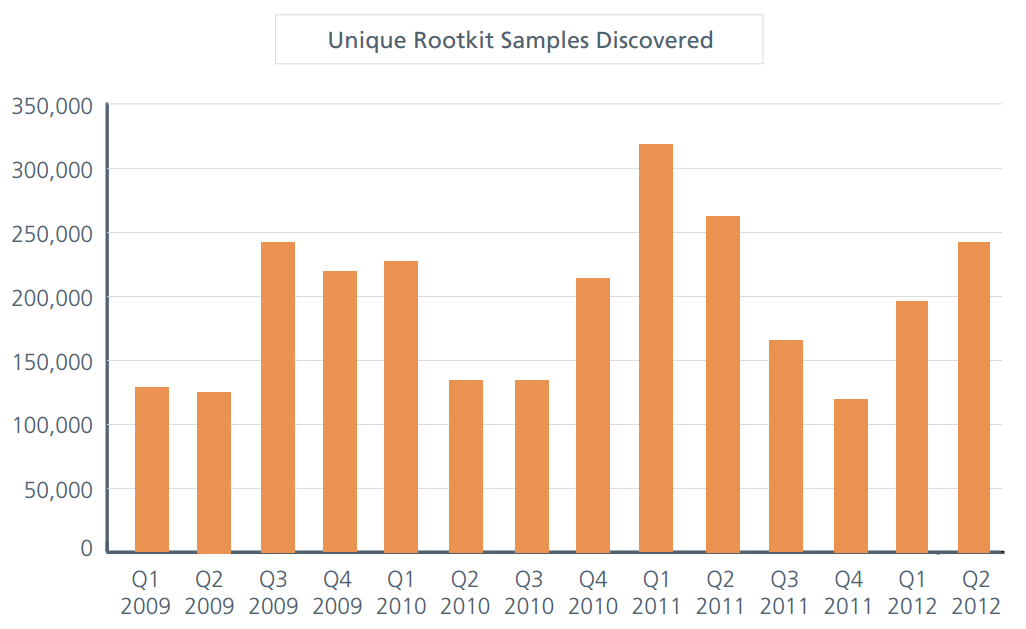
\includegraphics[scale=0.5]{figuras/graph-root.png}
  \caption{Amostras Rootkit �nicas Descobertas \cite{MCAFEE2012}}
  \label{fig:graph-root}
\end{figure}

Com um processo bem definido o perito tende a diminuir o tempo de an�lise e um melhor aproveitamento das mesmas.
Sendo assim, esse trabalho poder� ajudar a tra�ar um processo bem elaborado de trabalho que seja r�pida e eficiente sem deixar brechas que permitam ou ajudem a��es antiforenses provendo mais qualidade com mais precis�o.

\section{Objetivos}

% ---------------------------------------------------------------------------------------------------- %
% Que problemas o estudo do tema pode resolver? (PREPARA��O PAR AO PROBLEMA DE PESQUISA E OBJETIVO)}
% ---------------------------------------------------------------------------------------------------- %

Esse estudo pode ajudar a esclarecer diversos t�picos obscuros a respeito do que pode ser encontrado em investiga��es forenses computacionais quando o perito se v� diante de amea�as persistentes e elaboradas como um rootkit e consequentemente pode ajudar a resolver casos onde foram feitas antiforense.

\subsection{Objetivo Geral}

% ---------------------------------------------------------------------------------------------------- %
%					ORIENTA��ES
% ---------------------------------------------------------------------------------------------------- %
%	� necess�rio apresentar o objetivo geral da pesquisa, ou seja, a meta proposta para a investiga��o, 
% que deve ser coerente com a quest�o de pesquisa.
% ---------------------------------------------------------------------------------------------------- %

Apresentar um processo para an�lise \emph{post mortem} de computadores com Microsoft Windows e as principais t�cnicas antiforense que podem ser encontradas em cada fase do processo.

\subsection{Objetivo Espec�fico}

% ---------------------------------------------------------------------------------------------------- %
%					ORIENTA��ES
% ---------------------------------------------------------------------------------------------------- %
%	De forma complementar, os objetivos espec�ficos, tamb�m presentes nesse item, constituem as etapas 
% de trabalho que permitem alcan�ar o objetivo geral. Como os objetivos traduzem a��es que ser�o executadas 
% ao longo da pesquisa; a apresenta��o destes no texto requer a utiliza��o de verbos no infinitivo.
% ---------------------------------------------------------------------------------------------------- %
Segue os objetivos espec�ficos utilizados para alcan�ar o objetivo principal:

\begin{itemize}
  \item Apresentar o que � ci�ncia forense, para que serve a ci�ncia forense e a legisla��o que garante a exist�ncia do perito no Brasil;
  \item Expor o que � um rootkit, seu funcionamento e seus tipos;
  \item Mostrar o que � antiforense computacional categorizando seus tipos; e
  \item Apresentar um processo de an�lise de rootkit.
\end{itemize}
 
\section{Descri��o dos Cap�tulos}

Ao longo dos cap�tulos s�o desenvolvidos os conhecimentos para o entendimento do tema proposto, onde cada um foi dividido em um assunto espec�fico.

No cap�tulo \emph{Ci�ncia Forense Computacional}, ser� mostrado uma vis�o geral do que � a ci�ncia forense, como ela � aplicada na computa��o, o que � um perito forense computacional e o respaldo legal para sua atua��o.

No cap�tulo \emph{Rootkit}, conduz a uma vis�o do funcionamento de um rootkit, algumas t�cnicas para subverter os sistema, o que � um \emph{malware}, a origem do nome rootkit, o que significa ser o usu�rio \emph{root}, os objetivos do rootkit, suas premissas e sua defini��o.
Tamb�m ser� mostrado os tipos de rootkits e analisado duas categorias gerais que exemplificam como o rootkit pode se manter oculto.

Por fim no �ltimo cap�tulo \emph{An�lise de Rootkits}, ser� apresentado um processo de an�lise \emph{post mortem} com passos que ir�o mostrar em cada etapa o que deve ser feito, t�cnicas antiforense e o qu�o complicado e impactante ela �.

% \section{Metodologia}
% \section{descricao dos capitulos} 

%Peritos em sua nobre luta di�ria podem se deparar, em uma das suas pr�ximas empreitadas t�o ut�is para a sociedade, com algum artefato que tenham sido subvertido por algu�m com o mesmo ou um maior conhecimento do que o seu sobre o corpo de delito periciado.

%Portando em assuntos que fojem da mediocridade cotidiana e adentram nesse mundo instigante e revelador da an�lise de artefatos �nicos, se faz necess�rio que quanto maior o desafio, maior dever� ser a dedica��o e paix�o do perito.

% O perito deve precaver-se de supor que situa��es mais corriqueiras tenham s� e apenas a resposta mais obvia desse modo evitando que sejam subestimadas.
% Al�m do conhecimento t�cnico e de foro que se espera de um perito, compreender que existem t�cnicas sofisticadas para destruir e/ou dificultar acesso a provas no ambito computacional � de fundamental necessidade para qualquer perito. 
% A combina��o do uso de diversas t�cnicas avan�adas com maestria se mostra realmente desafiadora, pois quando isso ocorre o artefato investigado pode estar preparado para ser investigado removendo rastros e evitando a cri��o de evid�ncias.
  % desenvolvimento
    \chapter{Forense Computacional}
% o que � forense? para que serve forense? O que � computa��o forense?

A humanidade sempre teve assuntos divergentes, onde em outrora esses assuntos eram resolvidos com o mais forte ou hapto sobrepujando a vontade doutro, com o advento da civiliza��o se convencionou o uso de um mediador que em teoria deve ser alguem neutro.

Quando trata-se de assuntos de disputa de interesse, espera-se que o mediador busque e chegue o mais pr�ximo poss�vel da verdade antes de tomar uma decis�o. Hoje � dado esse poder de media��o ao juiz, contudo em diversos conflitos se faz necess�rio conhecimentos t�cnicos especificos. Nesses casos ele � auxiliado por um especialista ou perito no assunto t�cnico em discuss�o. Para tal, esse especialista utiliza-se da ci�ncia forense para trazer luz os fatos respaldando a decis�o do juiz sobre o assunto.

Segundo \citeonline{HOU} ci�ncia � um ``corpo de conhecimentos sistematizados adquiridos via observa��o, identifica��o, pesquisa e explica��o de determinadas categorias de fon�menos e fatos, e formulados met�dica e racionalmente.'' e forense � ``relativo aos tribunais e � justi�a''. Logo as ci�ncias forenses � a utiliza��o da ci�ncia ``� an�lise de vest�gios, no intuito de responder �s demandas judiciais'' \cite[p. -3 ]{CF}.

De certo a �rea m�dica foi a primeira a ser requisitada em tribunais construindo t�cnicas que levaram ao desenvolvimento ao longo dos anos da medicina legal. No Imp�rio Romano m�dicos eram chamados para lucidar mortes diz \citeonline{ML}, outro exemplo hist�rico da import�ncia do parecer t�cnico pode ser visto no \emph{C�digo Criminal Carolino} feito em 1532 por Carlos Magno que definia a an�lise m�dica em determinados crimes.

Com o avan�o da tecnologia e o valor da pespectiva especializada, foi natural que outras �reas tamb�m fossem utilizadas no foro. A computa��o forense, apesar da tecnologia e inova��o inatas, conceitualmente ainda se prop�e a grosso modo a usar a ci�ncia para mostrar fatos demandados judicialmente, como podemos ver em \citeonline{DCF2011}, ``[...] computa��o forense tem como objetivo principal determinar a din�mica, a materialidade e autoria de il�citos ligados � �rea da inform�tica, tendo como quest�o principal a identifica��o e o processamento de evid�ncias digitais em provas materiais [...], por m�todos t�cnicos-cient�ficos, conferindo-lhes validade probat�ria em ju�zo.''.

% citar legisla��o brasileiro sobre peritos e falar mais da hist�ria da computa��o forense
    \chapter{Antiforense Computacional}

\citeonline{RH2006} define antiforense como m�todo para prevenir ou agir contra a ci�ncia usada a favor das leis civis e criminais que s�o aplicadas pelos �rg�os como a pol�cia. J� \citeonline{BERI2007}, amplia essa ideia mostrando que � mais que uma t�cnica usada, � uma abordagem crimosa. Logo antiforense computacional pode ser definida como qualquer a��o praticada para obstruir, dificultar ou destruir evid�ncias ou provas no �mbito computacional.

Dentre as modalidades de antiforense computacional, \citeonline{BH2009} as categoriza em cinco grandes grupos, sendo eles: destrui��o de dados, oculta��o de dados, corrup��o de dados, fabrica��o de dados e elimina��o da fonte de dados.


    \chapter{Rootkits}

%%%%%%%%%%%%%%%%%%%%%%%%%%%%%%%%%%%%%%%%%%%%%%%%%%%%%%%%%%%%%%%%%%%%%%%
%				MALWARE					%
%%%%%%%%%%%%%%%%%%%%%%%%%%%%%%%%%%%%%%%%%%%%%%%%%%%%%%%%%%%%%%%%%%%%%%%
% Outros agentes infeciosos: O que n�o � um rootkit?

Malware � a jun��o das palavras em ingl�s \emph{malicious} e \emph{software}, termos em ingl�s que pode ser traduzido livremente como aplicativo malicioso. Dessa forma podemos considerar como malware os v�rus, worms, trojans, botnets kit dentro outros, contudo o inverso n�o � valido, ou seja, todo v�rus � um malware, mas nem todo malware � um v�rus.

% defini��o de malware, virus, botnet etc. \cite[p. 15]{BILL2009}. diferen�as entre worm e v�rus
% virus e worms, born to be spred
% 1980 - virus - floppy disk - display in to startup "Your computer is now stoned"
% 1988 - worm - Morris Worm
Os v�rus e worms s�o feitos para se espalha a diferen�a est� em como eles se espalham. O v�rus precisa ser ativado ou executado pelo usu�rio e em geral fica atrelado a algum executavel que pode ser ou n�o um programa legitimo subvertido \cite{MARK1995}, ao contr�rio do worm que n�o precisam da a��o direta do usu�rio para se espalhar e permanece apenas na mem�ria \cite{MCAFEE2013}.

% botnet zombies
Uma \emph{botnet} � uma rede de computadores controlados por cybercriminosos\cite{KAS2013}. Basicamente quando um computador � infectado pelo agente da \emph{botnet} o mesmo se torna parte da rede e � controlado pelo dono da botnet. 

%%%%%%%%%%%%%%%%%%%%%%%%%%%%%%%%%%%%%%%%%%%%%%%%%%%%%%%%%%%%%%%%%%%%%%%
%				ROOTKIT					%
%%%%%%%%%%%%%%%%%%%%%%%%%%%%%%%%%%%%%%%%%%%%%%%%%%%%%%%%%%%%%%%%%%%%%%%
% Defini��o: O que � rootkit?
No universo \emph{UNIX\footnote{Um sistema operacional multiusu�rio amplamente utilizado.}} ou \emph{UNIX-like\footnote{Sistemas Operacionais baseados no Unix, como o GNU/Linux}} a conta de usu�rio com menor restri��o de seguran�a � refer�nciada como conta \emph{root} sendo que em alguns sistemas o nome de usu�rio � literalmente root, mas isso � apenas uma conven��o hist�rica do que uma imposi��o \cite{BILL2009}. Enquanto \emph{kit} significa conjunto de pe�as \cite{DIING}. 

Rootkit pode ser visto como um ``kit'' composto de pequenos programas �teism por exemplo, bin�rios, scripts, arquivos de configura��o que permitem a um atacante manter o acesso ``root''. Em outras palavras, um rootkit � um conjunto de programas e de c�digo, que permite a presen�a permanente ou consistente, n�o detect�vel em um computador \cite{GREG2005}.

Essa cole��o de ferramentas que permitem aos invasores ocultarem suas atividades em um computador, de modo que eles podem secretamente monitorar e controlar o sistema por um per�odo prolongado, ou seja, existem tr�s servi�os que o s�o inerentes dos rootkits, oculta��o, comando e controle (C2) e vigil�ncia \cite{BILL2009}. Oculta��o, o rootkit deve passar despercebido, sem que o usu�rio e/ou antiv�rus o detecte; vigil�ncia ou monitoramento basicamente consiste em acompanhar as a��es do usu�rio, o rootkit tem que ser capaz de saber o que o usu�rio est� fazendo; e comando e controle, permite ao dono do rootkit o controle remoto sobre o mesmo, definindo suas a��es e direcionando. Desses tr�s servi�os o mais importante para o rootkit � a furtividade, pois um rootkit detect�vel vai durar muito pouco.

Como pode ser visto cada um desses agentes subversivos tem defini��es e caracter�sticas pr�prias diferentes e uma em comum todos eles subvertem o sistema de alguma forma, contudo � bom resaltar que nem todo rootkit � um malware, pois existem aplica��es leg�timas para o mesmo, como de computadores coorporativos e inclusive aplica��es investigativas.

%Historico
Os primeiros rootkits apareceram em de 20 anos atr�s no fim dos anos 80 e in�cio dos 90, quando alguns foram percebidos comportamentos anormais em computadores como espa�o em disco utilizado sem identifica��o, conex�es de rede n�o-listadas e uso anormal do CPU \cite{PR2011}.

% o que o rootkit execucar sem ser percebido? Isso � fundamental para entender onde e o que o rootkit pode estar fazendo
% hunk interrup��es
Basicamente o processador pode receber dois tipos de exce��es, uma gerada por hardware chamada de externa e interrup��es geradas por programas\cite[p. 6-2 Vol. 3A]{INT64IA322011}. A grosso modo, quando uma interrup��o ou exce��o ocorre o processador usa o endere�o de mem�ria armazenado no indice correspondente a interrup��o lan�ada que por defini��o aponta para uma \emph{procedure} que trata a interrup��o \cite{INT803861986}, ou seja, esse endere�o na mem�ria vai direcionar o processamento a \emph{procedure} especifica para a interrup��o ou exce��o que ocorreu. O rootkit pode interceptar uma chamada a tabela estrutura de dados com indices dessas tratativas como \emph{Interrupt Vector (IVT)} em modo real ou a \emph{Interrupt Descriptor Table (IDT)} em modo protegido, ambas as estruturas possuem fun��es similares, apesar da forma como trabalham ser muito distinta.

%pathing


% hook memory

tipos de rootkit http://www.terena.org/activities/tf-csirt/meeting27/oesterberg-rootkits.pdf

% Ir em cada referencia e verificar se foi usada

falando assim parece uma tarefa f�cil realizar qualquer um desses metodos...


% \begin{citacao}
% ``
% 1989: Primeiro alterador de logs � encontrado em sistemas corrompidos.
% 1994: Primeiros rootkits em sistemas operacionais da Sun s�o detectados.
% 1996: Primeiro rootkit para Linux aparece publicamente.
% 1997: Rootkits a n�vel de kernel (atrav�s de m�dulos carreg�veis pelo kernel) s�o propostos
% na ``Phrack''.
% 1998: Rootkits que se instalam em n�veis mais pr�ximos ao hardware s�o propostos por Silvio
% Cesare.
% 2000: Rootkit a n�vel de biblioteca � lan�ado.
% 2002: Fun��es de ``sniffers'' come�am a ser introduzidas em rootkits.
% 2005: SONY/BMG causam esc�ndalos ao incluir rootkit antipirataria em seus CDs
% 2006: A pesquisadora de seguran�a Joanna Rutkowska cria o Blue Pill, um rootkit a n�vel
% de m�quina virtual em hardware.
% 2007: Mebroot, um rootkit a n�vel de boot, � descoberto pela empresa de seguran�a iDefense.
% ''\cite[p. 13]{PR2011}
% \end{citacao}


%quem usa \cite[p. 13]{BILL2009}, usos para rootkit \cite{GREG2005} -> Why Do Rootkits Exist?

% Como ele pode subverter um sistema

% An�lise, detec��o e forense - montanaro.pdf

%bombas l�gicas


% Mostrar o que ele pode fazer usando se poss�vel com exemplos reais;
%resumo: rootkits com suas pr�ticas comuns e respectivos hist�ricos junto com algumas t�cnicas de subvers�o
%introdu��o: as pr�ticas mais comuns e como o rootkit pode ser usado na antiforense Como o rootkit pode impedir a forma��o de provas;

% \cite{PR2011} rootkit em bios e em outros lugares (onde o pode se esconder?) ou placa de video (eko)

Jamie Butler, the creator of the FU rootkit


O uso de rootkits � limitado a usu�rios avan�ados sendo que seu desenvolvimento exige conhecimentos profundos tanto de arquitetura de computadores quanto do funcionamento do Sistema Operacional que o mesmo vai corromper.










Rootkits proporcionam uma grande variedades de op��es e pode ser utilizado para quase tudo, 

vem sendo utilizado historicamente para subverter sistemas dando permiss�o 

O fato de alguns eventos e rootkits terem ficados famosos, como � o caso do stuxnet\cite{}, torna esse assunto muito interessante de ser abordado, porque 




A grosso modo rootkits sempre tentar�o esconder sua presen�a e seus rastros, logo a antiforense desde o inicio j� � parte ...

n�o s�o novidades e sua aplica��o j� n�o � 




e durante o avan�o do trabalho, poder�o ser notadas diversas formas de detec��o de rootkits al�m de ind�cios de seu uso em an�lises.

%     \chapter{An�lise}
Desenvolver em cima da an�lise do funcionamento do rootkit e do seu potencial fatores que devem ser levados em conta antes de qualquer an�lise; e
Contemplar o trabalho com um estudo de caso.
  %fim do desenvolvimento
  \chapter{Conclusão}
nao existe tecnica antiforense 100\% nem metodologia para analise infalivel, nem 100\% segura e confiavel. foi mostrado diversas técnicas para atrasar e confundir o perito, e por vezes tornando o tempo de análise tao grande que o mesmo nao poderia 


  % elementos p�s-textuais
  \bibliography{bb}
\bibliographystyle{abnt-alf}
  \include{glossario}
  \include{apendiceanexos}

\end{document}
